\documentclass[tikz,border=6pt]{standalone}
\usetikzlibrary{arrows.meta,positioning}
\begin{document}
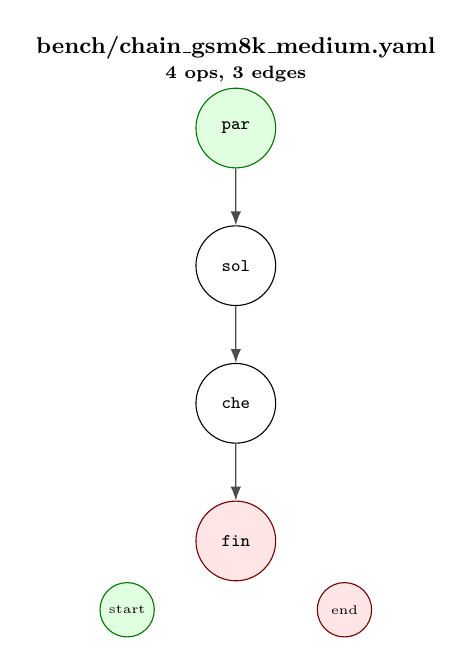
\begin{tikzpicture}[>=Latex, scale=0.92, transform shape,
  op/.style={circle, draw, align=center, minimum size=11mm, inner sep=0pt, font=\scriptsize, fill=white},
  start/.style={op, fill=green!12, draw=green!45!black},
  end/.style={op, fill=red!10, draw=red!45!black},
  startend/.style={op, fill=yellow!16, draw=orange!55!black},
  edge/.style={->, line width=0.45pt, draw=black!70}
]
\node[font=\small\bfseries, align=center] at (0,0.95) {bench/chain\_gsm8k\_medium.yaml\\[-1pt]{\scriptsize 4 ops, 3 edges}};
\node[start] (n0) at (0.00,0.00) {\texttt{par}};
\node[op] (n1) at (0.00,-1.90) {\texttt{sol}};
\node[op] (n2) at (0.00,-3.80) {\texttt{che}};
\node[end] (n3) at (0.00,-5.70) {\texttt{fin}};
\draw[edge] (n2) -- (n3);
\draw[edge] (n0) -- (n1);
\draw[edge] (n1) -- (n2);
\node[start, minimum width=0.75cm, minimum height=0.45cm, font=\tiny] at (-1.50,-6.65) {start};
\node[end, minimum width=0.75cm, minimum height=0.45cm, font=\tiny] at (1.50,-6.65) {end};
\end{tikzpicture}
\end{document}
